\documentclass{article}

\usepackage[russian]{babel}
\usepackage[utf8]{inputenc}
\usepackage{gensymb}
\usepackage{graphicx}
\usepackage{wrapfig}
\usepackage{mathtools}
\usepackage{tabularx}
\usepackage{subcaption}
\usepackage[
	labelfont = bf,
	labelsep = period,	
	justification = centering,
	textfont = sl
]{caption}
\usepackage[
	top = 2cm,
	bottom = 2cm,
	left = 3cm,
	right = 3cm
]{geometry}

\newcolumntype{C}[0]{>{\centering\arraybackslash}X}
\renewcommand\tabularxcolumn[1]{m{#1}}
\renewcommand{\theequation}{\thesection .\arabic{equation}}


\begin{document}
	\section{Обзор}
	\begin{wrapfigure}[12]{r}{0.4\textwidth}	
		\vspace{-1pc}	
		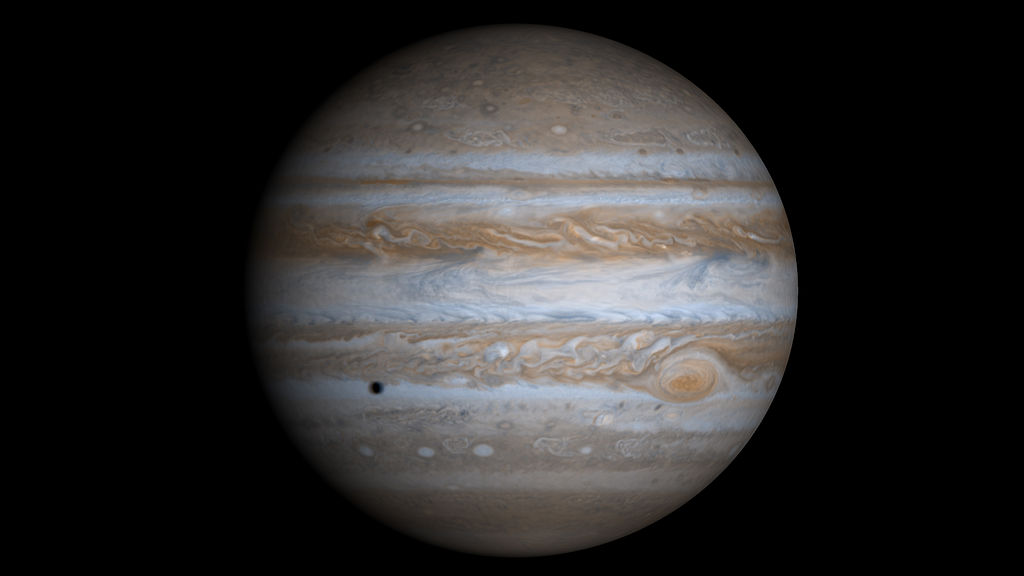
\includegraphics[width = 0.4\textwidth]{img/Jupiter}		
		\caption{Изображение Юпитера, созданное аппаратом Кассини}
		\label{pic:Jupiter}
	\end{wrapfigure}
	
    \textbf{Юпитер}~--- крупнейшая планета Солнечной системы, пятая по удалённости от Солнца. Наряду с
    Сатурном, Ураном и Нептуном, Юпитер классифицируется как \textit{газовый гигант}.
    
	Планета была известна людям с глубокой древности, что нашло своё отражение в мифологии и религиозных
	верованиях различных культур: месопотамской, вавилонской, греческой и других. Современное название
	Юпитера происходит от имени древнеримского верховного бога-громовержца.
	
	\begin{wrapfigure}{L}{0.3\textwidth}
		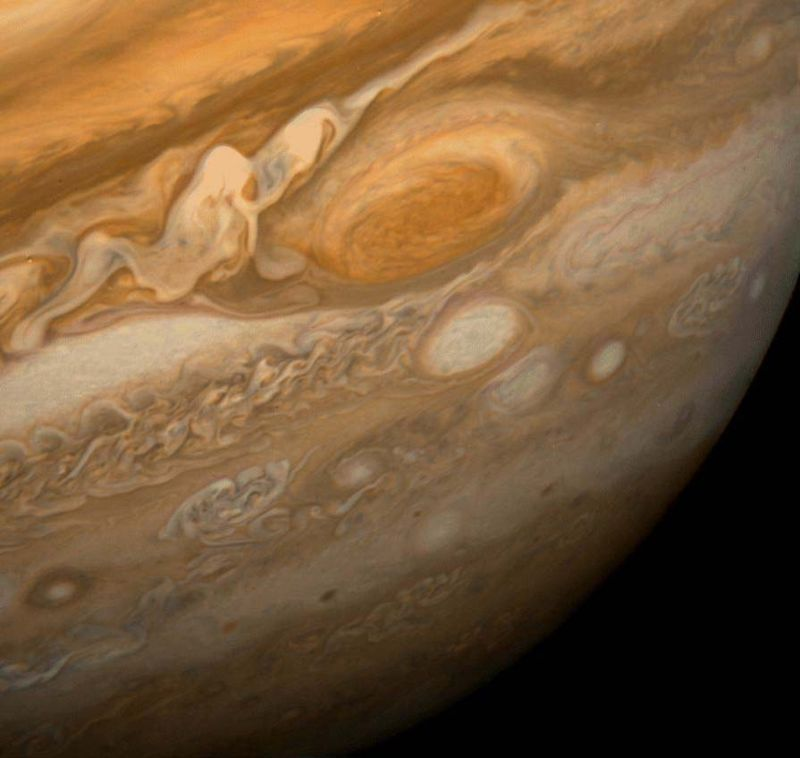
\includegraphics[width = 0.3\textwidth]{img/grs}
		\caption{Изображение Большого красного пятна}
		\label{pic:grs}
		\vspace{-1pc}
	\end{wrapfigure}	
	Ряд атмосферных явлений на Юпитере: штормы, молнии, полярные сияния, — имеет масштабы, на порядки
	превосходящие земные. Примечательным образованием в атмосфере является Большое красное пятно~---
	гигантский шторм, известный с XVII века (его изображение можно увидеть на рис.~\ref{pic:grs}).
	
	Юпитер имеет, по крайней мере, 79 спутников, самые крупные из которых — Ио, Европа, Ганимед и
	Каллисто — были открыты \textit{Галилео Галилеем} в 1610 году.

	Исследования Юпитера проводятся при помощи наземных и орбитальных телескопов; с 1970-х годов к
	планете было отправлено 8 межпланетных аппаратов НАСА: «Пионеры», «Вояджеры», «Галилео» и другие.

	Во время великих противостояний (одно из которых происходило в сентябре 2010 года) Юпитер
	виден невооружённым глазом как один из самых ярких объектов на ночном небосклоне после Луны и
	Венеры. Диск и спутники Юпитера являются популярными объектами наблюдения для астрономов-любителей,
	сделавших ряд открытий (например, кометы Шумейкеров-Леви, которая столкнулась с Юпитером в 1994 
	году, или исчезновения Южного экваториального пояса Юпитера в 2010 году)
	\section{Спутники}	
	На 2018 год известны 79 спутников Юпитера, несколько из которых являются \textit{нерегулярными}, 
	т.е.~движение которых отличается от движения обычных (естественных) спутников. Кроме того, у Юпитера
	есть и система колец. В СМИ, популярной и художественной литературе нередко называют лунами Юпитера.
	
	Первые спутники Юпитера были открыты еще в 1610 Галилео Галилеем. Они названы в честь древнегреческих
	богов~--- Ио, Каллисто, Европа и Ганимед. Интереснен тот факт, что имена им дал другой ученый того
	времени~--- Симон Мариус, который также претендовал на первенство открытия этих спутников.
	\begin{figure}[h!]
	\begin{tabularx}{\textwidth}{|C|C|C|C|C|}
		\hline
		Название & Масса (кг) & Большая полуось(км) & Орбитальный период (д) & Наклон орбиты\\		
		\hline
		Ио & $8.9\cdot 10^{22}$ & 421 700 & 1.77 & $0.050\degree$\\
		\hline
		Европа & $4.8\cdot10^{22}$ & 671 034 & 3.55 & $0.471\degree$\\
		\hline
		Ганимед & $1.5\cdot10^{23}$ & 1 070 412 & 7.15 & $0.204\degree$\\
		\hline
		Каллисто & $1.1\cdot10^{23}$ & 1 882 709 & 16.69 & $0.205\degree$\\
		\hline
	\end{tabularx}
	\end{figure}
	\section{Интегрирование}
	Пусть имеется некоторая непрерывная функция $f(x),$ заданная уравнением~(\ref{eq:func}):
	\begin{equation}
		f(x) = \begin{cases}
			-2, & x \leq -4;\\
			x^2 + 8x + 14, & -4 \leq x \leq -2;\\
			x + 4, & -2 \leq x \leq 0;\\
			4 - \frac{x^2}{\sqrt{3}}, & 0 \leq x \leq 6;\\
			\sin x, & x \geq 6.
		\end{cases}
		\label{eq:func}
	\end{equation}
	Производная данной функции также будет иметь вид кусочно-заданной функции, но она не будет
	непрерывной, разрывы будут наблюдаться в точках $(-2, -2)$, $(0, 4)$ и $(6, 0)$:
	\begin{equation}
		f'(x) = \begin{cases}
			0, & x \leq -4;\\
			2x + 8, & -4 \leq x < -2;\\
			1, & -2 < x < 0;\\
			-2\frac{x}{\sqrt{3}}, & 0 < x < 6;\\
			\cos x, & x > 6.
		\end{cases}
	\end{equation}	
	Попробуем проинтегрировать нашу функцию на отрезке $[-5, 7]$:
	\begin{multline}		
		\int\limits_{-5}^7 f(x)dx = \int\limits_{-5}^{-4} f(x)dx + \int\limits_{-4}^{-2} f(x)dx + 
			\int\limits_{-2}^0 f(x)dx + \int\limits_0^6 f(x)dx + \int\limits_6^7 f(x)dx =\\
		= \int\limits_{-5}^{-4} -2dx + \int\limits_{-4}^{-2} (x^2 + 8x + 14)dx + 
			\int\limits_{-2}^0 (x + 4)dx + \int\limits_0^6 \left(4 - \frac{x^2}{\sqrt{3}}\right)dx +
			\int\limits_6^7 \sin xdx = \\
		= -2x\bigg|_{-5}^{-4} + \frac{x^3}{3}\bigg|_{-4}^{-2} + 4x^2\bigg|_{-4}^{-2} + 
			14x\bigg|_{-4}^{-2} + \frac{x^2}{2}\bigg|_{-2}^{0} + 4x\bigg|_{-2}^{0} + 4x\bigg|_{0}^{6} -
			 \frac{x^3}{3\sqrt{3}}\bigg|_{0}^{6} - \cos x\bigg|_{6}^{7} =\\
		= -2\cdot(-4 + 5) + \frac{(-2)^3 - (-4)^3}{3} + 4\cdot\big((-2)^2 - (-4)^2\big) + 
		14\cdot\big((-2)-(-4)\big) +
		\frac{0^2 - (-2)^2}{2} + 4\cdot\big(0 - (-2)\big) + 4\cdot(6 - 0) -\\
		- \frac{6^3 - 0^3}{3\sqrt{3}} - (\cos 7 - \cos 6) = - 2 + 18.67 - 48 + 28 + 2 + 8 + 24 - 41.56 + 
		0.2 = -10.69
	\end{multline}
	\section{Затмения}
	Затмение~--- астрономическая ситуация, при которой одно небесное тело заслоняет свет от другого
	небесного тела.

	Наиболее известны лунные и солнечные затмения. Также существуют такие явления, как прохождения планет
	(Меркурия и Венеры) по диску Солнца.

	Частичное солнечное затмение. Когда Луна проходит между Землей и Солнцем, но не блокирует весь свет,
	это вызывает частичное солнечное затмение. Солнце выглядит в виде полумесячного диска.
	
	Полное солнечное затмение. Появляется, когда Луна находится на прямой линии между Землей и Солнцем
	полностью блокируя свет.
	
	Кольцеобразное затмение. Также появляется при нахождении на прямой линии между Землей и Солнцем, но
	блокирует не весь свет.
	
	Гибридное затмение. Это затмение - самое редкое. Оно появляется, когда Луна недостаточно близка к
	Земле во время начала и конца затмения.
	\begin{figure}[p]
		\centering
		\begin{subfigure}{0.3\textwidth}
			\centering
			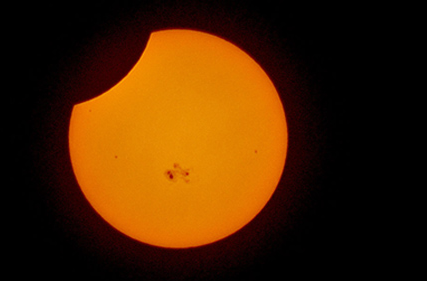
\includegraphics[scale = 0.4]{img/partial}
			\caption{Частичное затмение}
		\end{subfigure}\hspace{0.2\textwidth}
		\begin{subfigure}{0.3\textwidth}
			\centering
			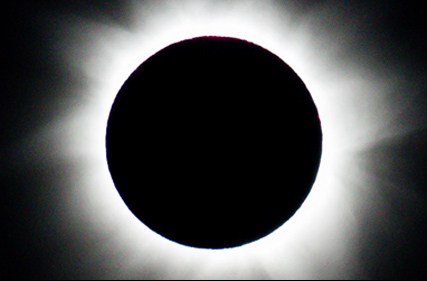
\includegraphics[scale = 0.4]{img/full}
			\caption{Полное затмение}		
		\end{subfigure}\\
		\begin{subfigure}{0.3\textwidth}
			\centering
			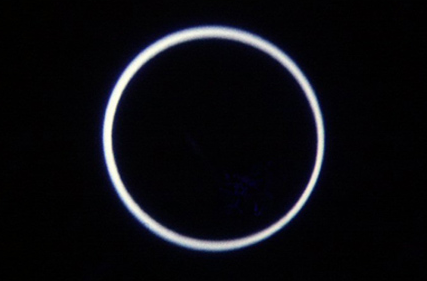
\includegraphics[scale = 0.4]{img/circle}
			\caption{Кольцевое затмение}
		\end{subfigure}\hspace{0.2\textwidth}
		\begin{subfigure}{0.3\textwidth}
			\centering
			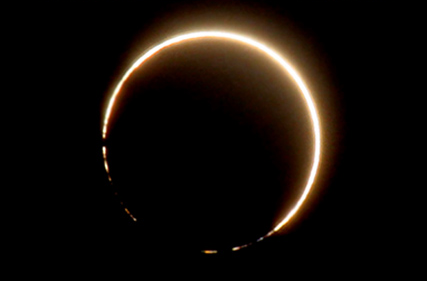
\includegraphics[scale = 0.4]{img/hybrid}
			\caption{Гибридное затмение}
		\end{subfigure}
		\caption{Фотографии затмений}
	\end{figure}
\end{document}